\chapter{Basic foundations of Inference}
\label{sectionBasicFoundationsForInference}
%\label{modeling}

%\section{Sampling Theory}
%\label{sectionSamplingTheory}



Statistical inference is concerned primarily with understanding the quality of parameter estimates. For example, a classic inferential question is, ``How sure are we that the estimated mean, $\bar{x}$, is near the true population mean, $\mu$?''
%We introduce these common themes in Sections~\ref{cltSection} and \ref{variabilityInEstimates} by discussing inference about the population mean, $\mu$, and set the stage for other parameters and scenarios in Section~\ref{aFrameworkForInference}. Some advanced considerations are discussed in Section~\ref{sampleSizeAndPower}. 
These are the questions that are answered in sections {\color{red}{REFERENCE}}
but at this point we set the stage for understanding the procedures behind these sections.
%Understanding 
A good familiarity with this chapter will make the rest of this book, and indeed the rest of statistics, seem much more familiar.
Sections~\ref{sectionSamplingDistribution}, \ref{cltSection} and \ref{variabilityInEstimates} all come together nicely in the example presented in case study~\ref{sectionCaseStudyChellyBlosson10MileRun}.
While the equations and details change depending on the setting, the foundations for inference are the same throughout all of statistics.


\section{Sampling distributions}
\label{sectionSamplingDistribution}

%\subsubsection{Sampling Distribution of the sample mean}

\index{point estimate|(}

In this section we discuss some background material that we use for  {\color{red}{Chapters~\ref{foundationsForInference},
~\ref{inferenceForNumericalData} and~\ref{inferenceForCategoricalData}.
The material in this section is not a rigorous exploration into sampling theory but it should
be sufficient enough for a good foundation to understand the material in Chapters~\ref{foundationsForInference},
~\ref{inferenceForNumericalData} and~\ref{inferenceForCategoricalData}. } }

We start with defining a point estimate.
A point estimate is a single value that can be regarded as the best guess of a parameter.

\begin{termBox}{\tBoxTitle{Point Estimate}
A \term{point estimate} is a a single value (i.e. a single point on the real number line) that
estimates the value of a parameter
}
\end{termBox}

A point estimate is obtained by choosing a suitable statistic that is calculated from sample data. 
The selected statistic is called the \term{point estimator} of the parameter.
For example the sample mean $\bar{x}$ is a point estimate of the population mean $\mu$,
and the sample standard deviation $s^{2}$ is a point estimate of $\sigma^{2}$ which is the population variance 
\footnote{note that there are other point estimators available $\sigma^{2}$ such as $\frac{(n-1)}{n}s^{2}$}.
Methods of finding point estimates such as maximum likelihood estimation and the method of moments
can be learnt in a course on mathematical statistics.

The next important term to define is \term{the sampling distribution}.
A sampling distribution is the distribution of a statistic.

\index{point estimate|)}

\begin{termBox}{\tBoxTitle{Sampling distribution}
The sampling distribution represents the distribution of the point estimates based on samples of a fixed size from a certain population. It is useful to think of a particular point estimate as being drawn from such a distribution. 
%Understanding the concept of a sampling distribution is central to understanding statistical inference.
}
\end{termBox}

Suppose we are interested in a certain population parameter $\theta$.
and our best guess of $\theta$ is point estimator $\hat{\theta}$.
%We are being completely general at this point and we are not specifying what $\theta$ is, but $\theta$ could be
%the population mean or the population median etc.
We are now interested in creating a sampling distribution for $\hat{\theta}$.
A sample of data of size $n$ is drawn from the population and a single instance of the estimator $\hat{\theta}_{1}$ is calculated from this sample data.
Another \term{independent sample} which is also size $n$ is drawn and another instance of the estimator $\hat{\theta}_{1}$ is calculated from this different sample data.
This process is repeated many times and we obtain a collection estimates
 $\hat{\theta}_{1}, \hat{\theta}_{2}, \ldots, \hat{\theta}_{m}$ where $m$ is very large; such as the order of several thousands\footnote{It is important to note that samples drawn are independent of one another. Whether samples are drawn with or without replacement usually does not matter since a population is typically very large.}.
We can now create a relative frequency distribution for the large collection of samples obtained.  
As $m$ approaches $\infty$ (i.e. we take an infinite number of samples and calculate a statistic for each one of these samples) the relative frequency distribution created for $\hat{\theta}$ 
is the sampling distribution of $\hat{\theta}$.
Figure~\ref{schematicSumamryOfSamplingDistribution} below gives
a summary of the manner in which a sampling distribution is created.


\begin{figure}[H]
\begin{center}
\hspace*{-1.50cm}	Population with parameter $\theta$
\end{center}

\begin{center}
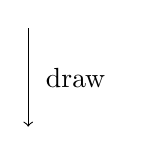
\begin{tikzpicture}
%\draw[thick,->] (0,0) -- (4.5,0);
\draw[->] (0,0) -- (0,-1.25);
\node [right] at (0.1,-0.625) {draw};
\end{tikzpicture}
\end{center}


\vspace{-0.25cm}

\begin{center}
\hspace*{-1.50cm}
\begin{tabular}{cccccccccc}
&	Sample 1	&	Sample 2		& Sample 3	& 	\quad$\cdots$\quad 	& \quad$\cdots$\quad & \quad$\cdots$\quad	\\
\ldelim\{{6}{3mm}[$n$\quad]	&	-		&	-			&	-		&	\quad$\cdots$\quad 	& \quad$\cdots$\quad & \quad$\cdots$\quad 	\\
&	-		&	-			&	-		&	\quad$\cdots$\quad 	& \quad$\cdots$\quad & \quad$\cdots$\quad 	\\
&	-		&	-			&	-		&	\quad$\cdots$\quad 	& \quad$\cdots$\quad & \quad$\cdots$\quad 	\\
&	\vdots	&	\vdots		&	\vdots	&	\quad$\vdots$\quad 	& \quad$\vdots$\quad & 
\quad$\vdots$\quad 	\\
&	-		&	-			&	-		&	\quad$\cdots$\quad 	& \quad$\cdots$\quad & \quad$\cdots$\quad 	\\
&	-		&	-			&	-		&	\quad$\cdots$\quad 	& \quad$\cdots$\quad & \quad$\cdots$\quad 	\\
\cline{2-7}
\hfill\\
statistic	&	$\hat{\theta}_{1}$	&	$\hat{\theta}_{2}$	&	$\hat{\theta}_{3}$	&	
\quad$\cdots$\quad & \quad$\cdots$\quad & \quad$\cdots$\quad \\
\end{tabular}
\end{center}


%\vspace{0.10cm}


\begin{center}
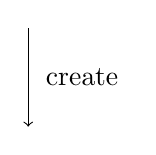
\begin{tikzpicture}
%\draw[thick,->] (0,0) -- (4.5,0);
\draw[->] (0,0) -- (0,-1.25);
\node [right] at (0.1,-0.625) {create};
\end{tikzpicture}
\end{center}


\begin{center}
\hspace*{-1.50cm}	Use $\hat{\theta}_{1}, \hat{\theta}_{2} \ldots, $ to create\\
\vspace{0.1cm}
\hspace*{-1.50cm}	the distribution for~ $\hat{\theta}$
\end{center}

\caption{Schematic summary on creating a sampling distribution for an estimator $\hat{\theta}$.}
\label{schematicSumamryOfSamplingDistribution}
\end{figure}


We use this framework to create a sampling distribution for the sample mean $\bar{x}$.
which is of particular interest to us.
In the next section we discuss a very important theorem related to the sample distributions which is the Central Limit Theorem.
The central limit theorem is used as a foundation for a lot of inference techniques.

%The sampling distribution of $\bar{x}$ is follows a normal distribution
%with a known mean and variance.


\section{Central Limit Theorem}
\label{cltSection}

%__________________
%\section{Examining the Central Limit Theorem}
%\label{cltSection}

\index{Central Limit Theorem|(}

The normal model for the sample mean tends to be very good when the sample consists of at least a sufficiently large number\footnote{The definition of ``sufficiently large'' is subjective. However we shall consider a sample size of $n \geq30$ to be large.} of independent observations and the population data are not strongly skewed. The Central Limit Theorem provides the theory that allows us to make this assumption.


\begin{termBox}{\tBoxTitle{Central Limit Theorem (CLT)}
Consider a random sample of size $n$ drawn from a population having mean $\mu$ and standard deviation $\sigma$. 
(The population may follow \underline{any} underlying distribution, however we know its mean
is $\mu$ and its standard deviation is $\sigma$).
%Consider a random sample of size $n$ drawn from a population (which follows \underline{any} distribution) having mean $\mu$ and standard deviation $\sigma$. 
%Suppose we take $m$ samples in this manner.
%When $m$ is large 
For sufficiently large $n$ the sampling distribution of the sample mean $\bar{x}$ is approximately normally distributed with a 
mean of $\mu_{\bar{x}} = \mu$ and standard deviation $\sigma_{\bar{x}} = \sigma / \sqrt{n}$
\begin{align*}
\bar{x}	~\stackrel{CLT}{\sim}~	N(\mu, \sigma/n)
\end{align*}
}
\end{termBox}


Stated informally, the central limit theorem states that the distribution of $\bar{x}$ is approximately normal
with mean $\mu$ and variance $\sigma/n$ where $n$ is the size of the sample drawn. 
%The approximation can be poor if the sample size is small, but it improves with larger sample sizes.
%\begin{termBox}{\tBoxTitle{Central Limit Theorem, informal definition}
%The distribution of $\bar{x}$ is approximately normal. The approximation can be poor if the sample size is small, but it improves with larger sample sizes.}
%\end{termBox}
%The Central Limit Theorem states that when the sample size is small, the normal approximation may not be very good. However, as the sample size becomes large, the normal approximation improves. We will investigate three cases to see roughly when the approximation is reasonable.
The population from which the samples are drawn can follow any distribution, however after
going through the procedure outlined in Figure~\ref{schematicSumamryOfSamplingDistribution},
the distribution of $\bar{x}$ will be normal.
Note that the approximation can be poor if %the sample size 
$n$ is small, but it improves with larger sample sizes\footnote{$n$ should not be confused with $m$ mentioned in~\ref{sectionSamplingDistribution}}.
%We will investigate three cases to see roughly when the approximation is reasonable.

The definition above is one way of stating the classical central limit theorem. 
We are not being extremely formal since the classical central limit theorem can be expressed 
in terms of $\bar{x}$ converging in distribution to $N(\mu, \sigma/\sqrt{n}$, however this
is something that is more suited for a course in statistical inference of mathematical statistics.
There are other ways of defining the central limit theorem and there are special forms of the central limit theorem such as the Lindeberg-Levy CLT, however the definition above is the most appropriate one for this course.

We will investigate three cases to see (roughly) when the approximation is reasonable.
We consider three data sets: one from a \emph{uniform} distribution, one from an \emph{exponential} distribution, and the other from a \emph{log-normal} distribution. These distributions are shown in the top panels of Figure~\ref{cltSimulations}. The uniform distribution is symmetric, the exponential distribution may be considered as having moderate skew since its right tail is relatively short (few outliers), and the log-normal distribution is strongly skewed and will tend to produce more apparent outliers.\index{skew!example: moderate}\index{skew!example: strong}

\begin{figure}[H]
   \centering
   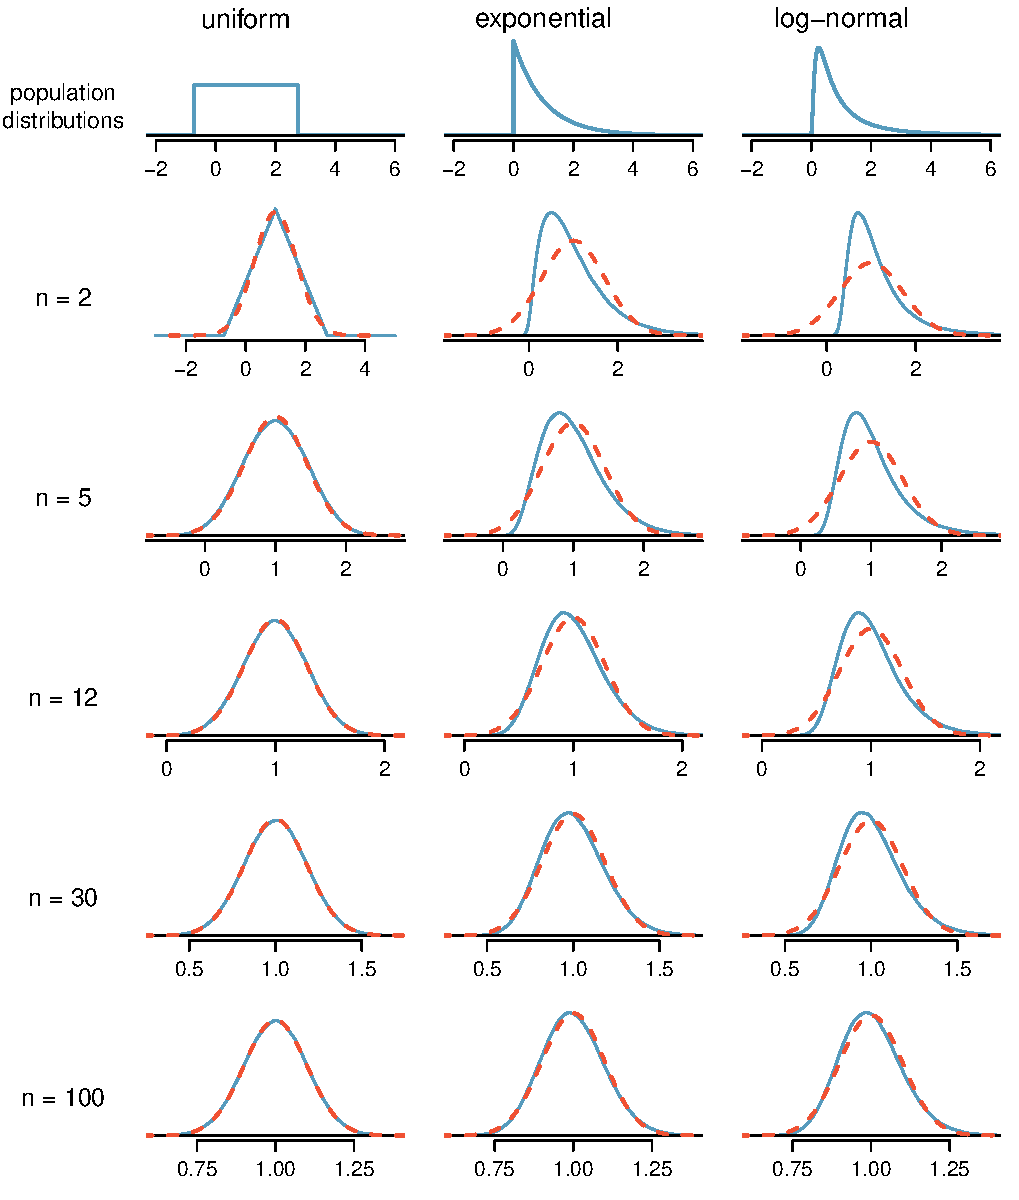
\includegraphics[width=\textwidth]{03-5/figures/cltSimulations/cltSimulationsNewest2.pdf}
   \caption{Sampling distributions for the mean at different sample sizes and for three different distributions. The dashed red lines show normal distributions.}
   \label{cltSimulations}
\end{figure}

The left panel in the $n=2$ row represents the sampling distribution of $\bar{x}$ if it is the sample mean of two observations from the uniform distribution shown. The dashed line represents the closest approximation of the normal distribution. Similarly, the center and right panels of the $n=2$ row represent the respective distributions of $\bar{x}$ for data from exponential and log-normal distributions.

\begin{exercise}
Examine the distributions in each row of Figure~\ref{cltSimulations}. What do you notice about the normal approximation for each sampling distribution as the sample size becomes larger?\footnote{The normal approximation becomes better as larger samples are used.}
\end{exercise}

\begin{example}{Would the normal approximation be good in all applications where the sample size is at least 30?}
Not necessarily. For example, the normal approximation for the log-normal example is questionable for a sample size of 30. Generally, the more skewed a population distribution or the more common the frequency of outliers, the larger the sample required to guarantee the distribution of the sample mean is nearly normal.
\end{example}

\begin{tipBox}{\tipBoxTitle{With larger $n$, the sampling distribution of $\bar{x}$ becomes more normal}
As the sample size increases, the normal model for $\bar{x}$ becomes more reasonable. 
%We can also relax our condition on skew when the sample size is very large.
}
\end{tipBox}

%We discussed in Section~\ref{seOfTheMean} that the sample standard deviation, $s$, could be used as a substitute of the population standard deviation, $\sigma$, when computing the standard error. This estimate tends to be reasonable when $n\geq30$. We will encounter alternative distributions for smaller sample sizes in Chapters~\ref{inferenceForNumericalData} and~\ref{inferenceForCategoricalData}.

\begin{example}{Figure~\ref{pokerProfitsCanApplyNormalToSampMean} shows a histogram of 50 observations. 


\begin{figure}[H]
   \centering
   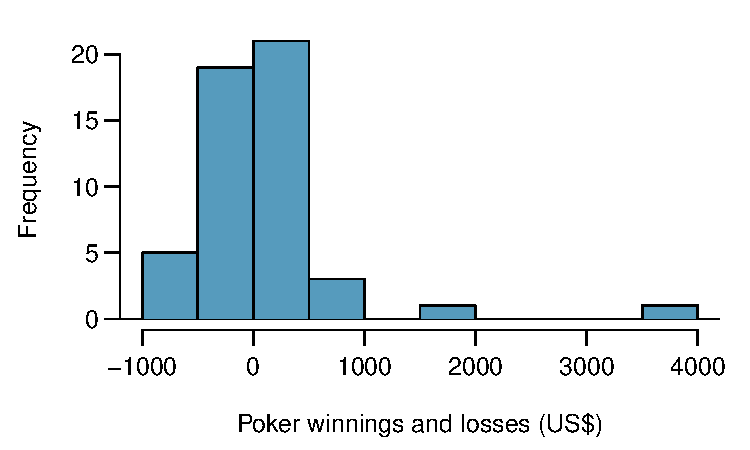
\includegraphics[height=58mm]{04/figures/pokerProfitsCanApplyNormalToSampMean/pokerProfitsCanApplyNormalToSampMean}
   \caption{Sample distribution of poker winnings. These data include some very clear outliers. These are problematic when considering the normality of the sample mean. For example, outliers are often an indicator of very strong skew\index{skew!example: very strong}.}
   \label{pokerProfitsCanApplyNormalToSampMean}
\end{figure}



These represent winnings and losses from 50 consecutive days of a professional poker player. Can the normal approximation be applied to the sample mean, 90.69?}
We should consider each of the required conditions.
\begin{itemize}
\setlength{\itemsep}{0mm}
\item[(1)] These are referred to as \term{time series data}, because the data arrived in a particular sequence. If the player wins on one day, it may influence how she plays the next. To make the assumption of independence we should perform careful checks on such data. While the supporting analysis is not shown, no evidence was found to indicate the observations are not independent.
\item[(2)] The sample size is 50, satisfying the sample size condition.
\item[(3)] There are two outliers, one very extreme, which suggests the data are very strongly skewed or very distant outliers may be common for this type of data. Outliers can play an important role and affect the distribution of the sample mean and the estimate of the standard error.
\end{itemize}
Since we should be skeptical of the independence of observations and the very extreme upper outlier poses a challenge, we should not use the normal model for the sample mean of these 50 observations. If we can obtain a much larger sample, perhaps several hundred observations, then the concerns about skew and outliers would no longer apply.
\end{example}

%\begin{figure}[ht]

\begin{caution}
{Examine data structure when considering independence}
{Some data sets are collected in such a way that they have a natural underlying structure between observations, e.g. when observations occur consecutively. Be especially cautious about independence assumptions regarding such data sets.}
\end{caution}

\begin{caution}
{Watch out for strong skew and outliers}
{Strong skew is often identified by the presence of clear outliers. If a data set has prominent outliers, or such observations are somewhat common for the type of data under study, then it is useful to collect a sample with many more than 30 observations if the normal model will be used for $\bar{x}$. There are no simple guidelines for what sample size is big enough for all situations, so proceed with caution when working in the presence of strong skew or more extreme outliers.}
\index{skew!strongly skewed guideline}
\index{Central Limit Theorem|)}
\end{caution}





\section{Variability in point estimates}
\label{variabilityInEstimates}
%\label{sectionVariabilityInPointEstimates}

The problem with point estimates is that they are usually not exactly equal to 
the value of the population parameter they are estimating.
Due to the nature of randomness the chances are that the point estimate taken from
a single sample will not be exact equal to the population parameter of interest.
It is important to note that the value of the population parameter stays fixed although
the value of point estimates drawn from samples can vary.

\begin{termBox}{\tBoxTitle{Parameter values do not vary}
We assume that the value of a population parameter remains fixed.}
\end{termBox}

For example, if we are interested in the mean height of all students at a university 
with a population of 20,000 students.
We assume that the true mean height of the 20,000 students is some fixed value that does not change.
Suppose we take a random sample of 30 students and measure the heights of these students.
There is a good chance that the mean of the 30 students will not be exact equal
to the mean of all 20,000 students.
As we increase our sample size then our estimate will become a better approximation of the
true parameter.
Going back to our example of measuring student height, suppose we calculated a sample mean
with the 100 students instead of 30. The sample mean based on 100 students is a better
approximation of the true population mean.

The way that we can quantify the amount of uncertainty of an estimator is with the
\term{standard error} of the estimator.

%We can see that the sample mean has some variability around the population mean, which can be quantified using the standard deviation of this distribution of sample means: $\sigma_{\bar{x}} = 1.59$. The standard deviation of the sample mean tells us how far the typical estimate is away from the actual population mean, 94.52 minutes. It also describes the typical \term{error} of the point estimate, and for this reason we usually call this standard deviation the \term{standard error (SE)}\index{SE}\marginpar[\raggedright\vspace{-4mm}
%
%$SE$\\\footnotesize standard\\error]{\raggedright\vspace{-4mm}
%
%$SE$\\\footnotesize standard\\error} of the estimate.

\begin{termBox}{\tBoxTitle{Standard error of an estimator}
The standard deviation associated with an estimate is called the \emph{standard error}. It describes the typical error or uncertainty associated with the estimate.}
\end{termBox}

The standard error is the standard deviation of the sampling distribution of the statistic of interest.
The calculation of the standard error depends on the situation.
For instance lets go back to the central limit theorem in Section~\ref{cltSection}.
We saw that the sampling distribution for the sample mean $\bar{x}$ 
is a normal distribution with mean $\mu$ and variance $\sigma^{2}/\sqrt{n}$.
Therefore the standard deviation of the sampling distribution of $\bar{x}$
is $\sigma/\sqrt{n}$
which means that the standard error of the mean is $\sigma/\sqrt{n}$.

We will learn the standard error of different point estimates in Chapters {\color{red}{REFERENCE}}
of this text.

%When considering the case of the point estimate $\bar{x}$, there is one problem: there is no obvious way to estimate its standard error from a single sample. However, statistical theory provides a helpful tool to address this issue. 








%__________________
\section{Case study: Cherry blosson 10 mile run}
\label{sectionCaseStudyChellyBlosson10MileRun}
%\label{variabilityInEstimates}


\index{data!run10|(}

We will illustrate the central limit theorem using a case study with with real data.
Throughout the next few sections we consider a data set called \data{run10}, which represents all 16,924 runners who finished the 2012 Cherry Blossom 10 mile run in Washington, DC.\footnote{\urlwofont{http://www.cherryblossom.org}} Part of this data set is shown in Table~\ref{run10DF}, and the variables are described in Table~\ref{run10Variables}.

\begin{table}[h]
\centering
\begin{tabular}{rrrrr}
  \hline
ID & time & age & gender & state \\ 
  \hline
1 & 92.25 & 38.00 & M & MD \\ 
2 & 106.35 & 33.00 & M & DC \\ 
3 & 89.33 & 55.00 & F & VA \\ 
4 & 113.50 & 24.00 & F & VA \\ 
$\vdots$ & $\vdots$ & $\vdots$ & $\vdots$ & $\vdots$ \\
16923 & 122.87 & 37.00 & F & VA \\ 
16924 & 93.30 & 27.00 & F & DC \\ 
   \hline
\end{tabular}
\caption{Six observations from the \data{run10} data set.}
\label{run10DF}
\end{table}
% library(openintro); library(xtable); data(run10); xtable(run10[c(1,2,3,4, nrow(run10)-1:0), c("time", "age", "gender", "state")])

\begin{table}[H]
\centering\small
\begin{tabular}{l p{65mm}}
\hline
{\bf variable} & {\bf description} \\
\hline
\var{time} & Ten mile run time, in minutes \\
\var{age} & Age, in years \\
\var{gender} & Gender (\resp{M} for male, \resp{F} for female) \\
\var{state} & Home state (or country if not from the US) \\
\hline
\end{tabular}
\caption{Variables and their descriptions for the \data{run10} data set.}
\label{run10Variables}
\end{table}

%\index{data!run10Samp|(}

These data are special because they include the results for the entire population of runners who finished the 2012 Cherry Blossom Run. 
We took a simple random sample of 
100 observations from
this population, which is represented in Table~\ref{run10SampDF}. We will use this sample, which we refer to as the \data{run10Samp} data set, to draw conclusions about the entire population. This is the practice of statistical inference in the broadest sense. Two histograms summarizing the time and age variables in the \data{run10Samp} data set are shown in Figure~\ref{run10SampHistograms}.

\begin{table}[H]
\centering
\begin{tabular}{crrccc}
  \hline
Sample 		& ID & time 	& age 	& gender 	& state 	\\ 
observation	&	&		&		&		&		\\
\hline
1 & 1983 & 88.31 & 59 & M & MD \\ 
2 & 8192 & 100.67 & 32 & M & VA \\ 
3 & 11020 & 109.52 & 33 & F & VA \\ 
$\vdots$ &  $\vdots$~~ &   $\vdots$~~~ &   $\vdots$~ &   $\vdots$~ &   $\vdots$~\, \\ 
100 & 1287 & 89.49 & 26 & M & DC \\ 
   \hline
\end{tabular}

%\begin{tabular}{rrrrr}
%  \hline
%ID & time & age & gender & state \\ 
%  \hline
%1983 & 88.31 & 59 & M & MD \\ 
%8192 & 100.67 & 32 & M & VA \\ 
%11020 & 109.52 & 33 & F & VA \\ 
%  $\vdots$~~ &   $\vdots$~~~ &   $\vdots$~ &   $\vdots$~ &   $\vdots$~\, \\ 
%1287 & 89.49 & 26 & M & DC \\ 
%   \hline
%\end{tabular}
\caption{Four observations for the \data{run10Samp} data set, which represents a simple random sample of 100 runners from the 2012 Cherry Blossom Run.}
\label{run10SampDF}
%library(openintro); library(xtable); data(run10); data(run10Samp); xtable(run10Samp[c(1,2,3,100),])
\end{table}

% WARNING: This figure is referenced in Section 4.2
\begin{figure}[H]
\centering
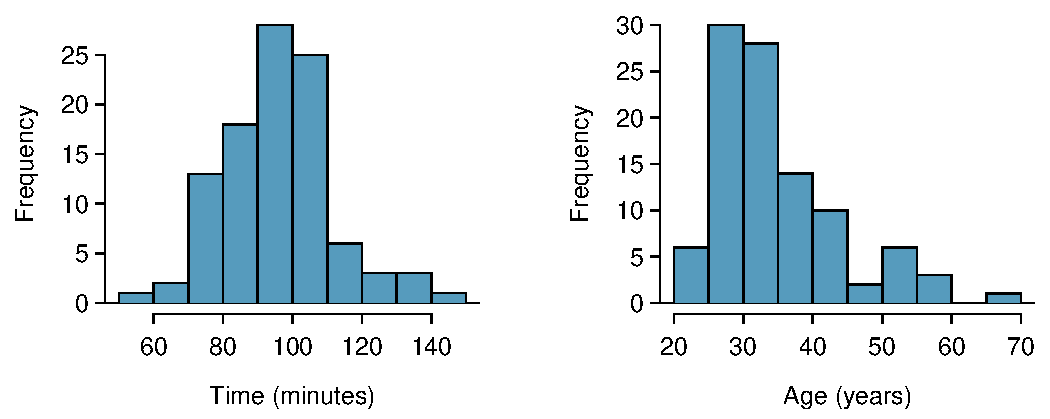
\includegraphics[width=\textwidth]{04-5/figures/run10SampHistograms/run10SampHistograms} 
\caption{Histograms of \var{time} and \var{age} for the sample Cherry Blossom Run data. The average time is in the mid-90s, and the average age is in the mid-30s. The age distribution is moderately skewed to the right.\index{skew!example: moderate}}
\label{run10SampHistograms}
\end{figure}







\index{point estimate|(}

We would like to estimate two features of the Cherry Blossom runners using the sample. 
\begin{itemize}
\setlength{\itemsep}{0mm}
\item[(1)] How long does it take a runner, on average, to complete the 10 miles?
\item[(2)] What is the average age of the runners?
\end{itemize}
These questions may be informative for planning the Cherry Blossom Run in future years.\footnote{While we focus on the mean in this chapter, questions regarding variation are often just as important in practice. For instance, we would plan an event very differently if the standard deviation of runner age was 2 versus if it was 20.} We will use $x_1, ..., x_{100}$ to represent the 10 mile time for each runner in our sample, and $y_1, ..., y_{100}$ will represent the age of each of these participants.

\subsection{Calculations of the sample mean}
\label{pointEstimates}

\index{point estimate!single mean|(}

We want to estimate the \term{population mean} based on the sample. The most intuitive way to go about doing this is to simply take the \term{sample mean}. That is, to estimate the average 10 mile run time of all participants, take the average time for the sample:
\begin{eqnarray*}
\bar{x} = \frac{88.22 + 100.58 + \dots + 89.40}{100} = 95.61
\end{eqnarray*}
The sample mean $\bar{x} = 95.61$ minutes a \term{point estimate} of the population mean.
%if we can only choose one value to estimate the population mean, this is our best guess. 
Suppose we take a new sample of 100 people and recompute the mean; we will probably not get the exact same answer that we got using the \data{run10Samp} data set. Estimates generally vary from one sample to another, and this \term{sampling variation} suggests our estimate may be close, but it will not be exactly equal to the parameter.

We can also estimate the average age of participants by examining the sample mean of \var{age}:
\begin{eqnarray*}
\bar{y} = \frac{59 + 32 + \dots + 26}{100} = 35.05
\end{eqnarray*}
%library(openintro); library(xtable); data(run10); data(run10Samp); run10Samp$age[c(1,2,100)]; mean(run10Samp$age); mean(run10$age, na.rm=TRUE)

What about generating point estimates of other \term{population parameters}, such as the population median or population standard deviation? Once again we might estimate parameters based on sample statistics, as shown in Table~\ref{ptEstimatesNetTimeAge}. For example, we estimate the population standard deviation for the running time using the sample standard deviation, 15.78 minutes.

\begin{table}[h]
\centering
\begin{tabular}{ l rr}
\hline
\resp{time}		& estimate & parameter  \\
\hline
mean		& 95.61 & 94.52 \\
median	& 95.46 & 94.03 \\
st. dev.		& 15.78 & 15.93 \\
\hline
\end{tabular}
\caption{Point estimates and parameter values for the \var{time} variable.}
\label{ptEstimatesNetTimeAge}
\end{table}
%library(openintro); library(xtable); data(run10); data(run10Samp); d <- run10Samp$time; mean(d); median(d); sd(d); d <- run10$time; mean(d); median(d); sd(d)


\begin{exercise} \label{pointEstimateOfDifferentNetTimesBetweenGender}
Suppose we want to estimate the difference in run times for men and women. If $\bar{x}_{men} = 87.65$ and $\bar{x}_{women} = 102.13$, then what would be a good point estimate for the population difference?\footnote{We could take the difference of the two sample means: $102.13 - 87.65 = 14.48$. Men ran about 14.48 minutes faster on average in the 2012 Cherry Blossom Run.}
\end{exercise}
%library(openintro); library(xtable); data(run10); data(run10Samp); (x <- by(run10Samp$time, run10Samp$gender, mean)); diff(x)

\begin{exercise}
If you had to provide a point estimate of the population IQR for the run time of participants, how might you make such an estimate using a sample?\footnote{To obtain a point estimate of the IQR for the population, we could take the IQR of the sample.}

\index{point estimate!single mean|)}

\end{exercise}

%\subsection{Point estimates are not exact}

As mentioned in Section~\ref{variabilityInEstimates}
point estimates are usually not exactly equal to the truth, but they get better as more data become available. We can see this by plotting a running mean from our \data{run10Samp} sample. A \term{running mean} is a sequence of means, where each mean uses one more observation in its calculation than the mean directly before it in the sequence. For example, the second mean in the sequence is the average of the first two observations and the third in the sequence is the average of the first three. The running mean for the 10 mile run time in the \data{run10Samp} data set is shown in Figure~\ref{netTimeRunningMean}, and it approaches the true population average, 94.52 minutes, as more data become available.

\begin{figure}[H]
   \centering
   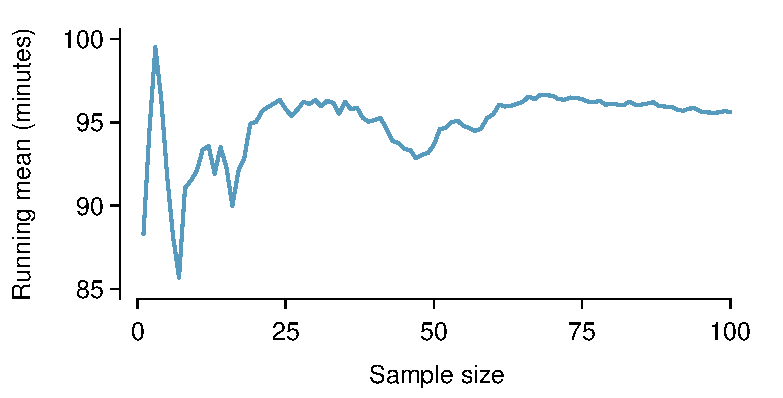
\includegraphics[width=0.7\textwidth]{04-5/figures/netTimeRunningMean/netTimeRunningMean}
   \caption{The mean computed after adding each individual to the sample. The mean tends to approach the true population average as more data become available.}
   \label{netTimeRunningMean}
\end{figure}

Sample point estimates only approximate the population parameter, and they vary from one sample to another. If we took another simple random sample of the Cherry Blossom runners, we would find that the sample mean for the run time would be a little different. It will be useful to quantify how variable
an estimate is from one sample to another. If this variability is small (i.e. the sample mean doesn't change much from one sample to another) then that estimate is probably very accurate. If it varies widely from one sample to another, then we should not expect our estimate to be very good.






\subsection{A sampling distribution of the sample mean}
%\label{sectionSamplingDistributionOfTheSampleMean}

From the random sample represented in \data{run10Samp}, we guessed the average time it takes to run 10 miles is 95.61 minutes. Suppose we take another random sample of 100 individuals and take its mean: 95.30 minutes. Suppose we took another (93.43 minutes) and another (94.16 minutes), and so on. If we do this many many times -- which we can do only because we have the entire population data set -- we can build up a \term{sampling distribution} for the sample mean when the sample size is 100, shown in Figure~\ref{netTime1000SamplingDistribution}.

\begin{figure}[H]
   \centering
   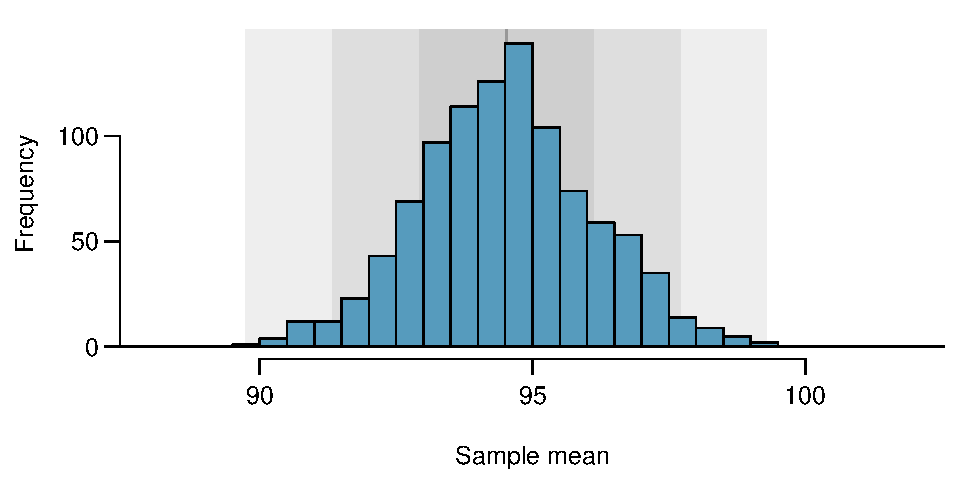
\includegraphics[width=0.7\textwidth]{04-5/figures/netTime1000SamplingDistribution/netTime1000SamplingDistribution}
   \caption{A histogram of 1000 sample means for run time, where the samples are of size $n=100$.}
   \label{netTime1000SamplingDistribution}
\end{figure}


%In Section~\ref{seOfTheMean}, we introduced a sampling distribution for $\bar{x}$, the average run time for samples of size 100.
%We examined this distribution earlier in Figure~\ref{netTime1000SamplingDistribution}. 
In Figure~\ref{netTime1000SamplingDistribution} we have introduced a sampling distribution for $\bar{x}$, the average run time for samples of size 100.
The shape of the distribution looks fairly normal with 1000 samples each of size 100.
Now we'll take 100,000 samples, calculate the mean of each, and plot them in a histogram to get an especially accurate depiction of the sampling distribution. This histogram is shown in the left panel of Figure~\ref{netTimeBigSamplingDistribution}.

%\begin{figure}[hht]
\begin{figure}[H]
   \centering
   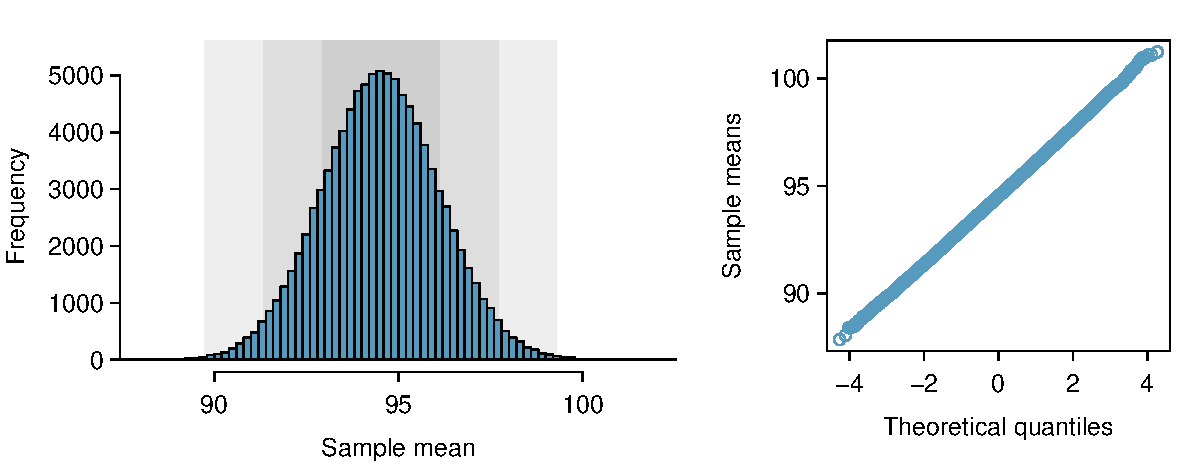
\includegraphics[width=\textwidth]{04-5/figures/netTimeBigSamplingDistribution/netTimeBigSamplingDistribution}
   \caption{The left panel shows a histogram of the sample means for 100,000 different random samples. The right panel shows a normal probability plot of those sample means.}
   \label{netTimeBigSamplingDistribution}
\end{figure}

%Let's increase the process further to 1,000,000 samples.
%Again we will calculate the mean for each sample and plot the frequency histogram for
%these 1,000,000 samples\footnote{The increase in the number of samples from 100 to 100,000 and to 1,000,000 is what we mean by $m \longrightarrow \infty$ in Section~\ref{sectionSamplingDistribution}.}.
%The result is in figure


Does this distribution look familiar? Hopefully so! The distribution of sample means closely resembles the normal distribution (see Section~\ref{normalDist}). A normal probability plot of these sample means is shown in the right panel of Figure~\ref{netTimeBigSamplingDistribution}. Because all of the points closely fall around a straight line, we can conclude the distribution of sample means is nearly normal. This result can be explained by the Central Limit Theorem.











\subsection{Standard error of the mean}
\label{seOfTheMean}

%From the random sample represented in \data{run10Samp}, we guessed the average time it takes to run 10 miles is 95.61 minutes. Suppose we take another random sample of 100 individuals and take its mean: 95.30 minutes. Suppose we took another (93.43 minutes) and another (94.16 minutes), and so on. If we do this many many times -- which we can do only because we have the entire population data set -- we can build up a \term{sampling distribution} for the sample mean when the sample size is 100, shown in Figure~\ref{netTime1000SamplingDistribution}.
%
%\begin{figure}[H]
%   \centering
%   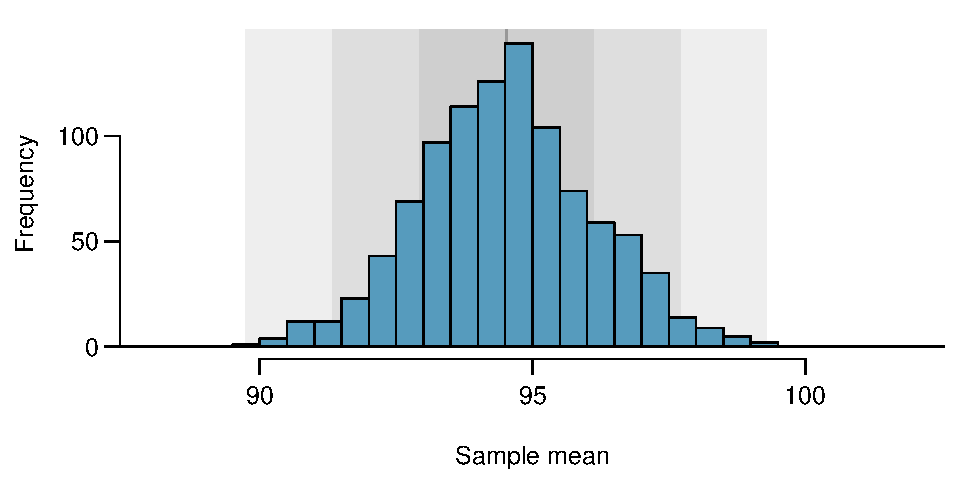
\includegraphics[width=0.7\textwidth]{04-5/figures/netTime1000SamplingDistribution/netTime1000SamplingDistribution}
%   \caption{A histogram of 1000 sample means for run time, where the samples are of size $n=100$.}
%   \label{netTime1000SamplingDistribution}
%\end{figure}

%\begin{termBox}{\tBoxTitle{Sampling distribution}
%The sampling distribution represents the distribution of the point estimates based on samples of a fixed size from a certain population. It is useful to think of a particular point estimate as being drawn from such a distribution. Understanding the concept of a sampling distribution is central to understanding statistical inference.}
%\end{termBox}

The sampling distribution shown in Figure~\ref{netTime1000SamplingDistribution} is unimodal and approximately symmetric. It is also centered exactly at the true population mean: $\mu=94.52$. Intuitively, this makes sense. The sample means should tend to ``fall around'' the population mean.

%We can see that the sample mean has some variability around the population mean, which can be quantified using the standard deviation of this distribution of sample means: $\sigma_{\bar{x}} = 1.59$. The standard deviation of the sample mean tells us how far the typical estimate is away from the actual population mean, 94.52 minutes. It also describes the typical \term{error} of the point estimate, and for this reason we usually call this standard deviation the \term{standard error (SE)}\index{SE}\marginpar[\raggedright\vspace{-4mm}
%
%$SE$\\\footnotesize standard\\error]{\raggedright\vspace{-4mm}
%
%$SE$\\\footnotesize standard\\error} of the estimate.
%
%\begin{termBox}{\tBoxTitle{Standard error of an estimate}
%The standard deviation associated with an estimate is called the \emph{standard error}. It describes the typical error or uncertainty associated with the estimate.}
%\end{termBox}
%
%When considering the case of the point estimate $\bar{x}$, there is one problem: there is no obvious way to estimate its standard error from a single sample. However, statistical theory provides a helpful tool to address this issue. 

\begin{exercise}\label{exerciseUsingseOfXBar}
(a) Would you rather use a small sample or a large sample when estimating a parameter? Why? (b) Using your reasoning from (a), would you expect a point estimate based on a small sample to have smaller or larger standard error than a point estimate based on a larger sample?\footnote{(a) Consider two random samples: one of size 10 and one of size 1000. Individual observations in the small sample are highly influential on the estimate while in larger samples these individual observations would more often average each other out. The larger sample would tend to provide a more accurate estimate. (b) If we think an estimate is better, we probably mean it typically has less error. Based on (a), our intuition suggests that a larger sample size corresponds to a smaller standard error.}
\end{exercise}

In the sample of 100 runners, the standard error of the sample mean is equal to one-tenth of the population standard deviation: $1.59 = 15.93/10$. In other words, the standard error of the sample mean based on 100 observations is equal to
\begin{eqnarray*}
SE_{\bar{x}} = \sigma_{\bar{x}} = \frac{\sigma_{x}}{\sqrt{n}} = \frac{15.93}{\sqrt{100}} = 1.59
\end{eqnarray*}
where $\sigma_{x}$ is the standard deviation of the individual observations. 
This is no coincidence; 
%We can show mathematically that this equation is correct when the observations are independent using the 
it is a direct result of using the central limit theorem and the probability tools of Section~\ref{randomVariablesSection}.

%\begin{termBox}{\tBoxTitle{Computing SE for the sample mean}
%Given $n$ independent observations from a population with standard deviation $\sigma$, the standard error of the sample mean is equal to \vspace{-1mm}
%\begin{eqnarray}
%SE = \frac{\sigma}{\sqrt{n}}
%\label{seOfXBar}
%\end{eqnarray}\vspace{-3mm}%
%
%A reliable method to ensure sample observations are independent is to conduct a simple random sample consisting of less than 10\% of the population.\index{standard error!single mean}
%}
%\end{termBox}


%There is one subtle issue of Equation~(\ref{seOfXBar}): the population standard deviation is typically unknown. You might have already guessed how to resolve this problem: we can use the point estimate of the standard deviation from the sample. This estimate tends to be sufficiently good when the sample size is at least 30 and the population distribution is not strongly skewed%\footnote{Some books suggest 30 is sufficient; we take a slightly more conservative approach.}
%% x <- c(); for(i in 1:10000){ x[i] <- mean(exp(rnorm(30, sd=0.5))) }; hist(x); (quantile(x, c(0.025, 0.975)) - mean(x)) / sd(x)
%% M <- mean(x); x <- rep(NA, 1000); for(i in 1:1000){ temp <- exp(rnorm(30, sd=0.5)); x[i] <- (max(temp) - M) / sd(temp) }; hist(x); quantile(x, 0.95)
%% for(i in 1:1000){ temp <- exp(rnorm(30, sd=0.5)); hist(temp, breaks=seq(0, 12, 0.5), main=round((max(temp) - mean(temp))/sd(temp), 1)); Sys.sleep(0.5) }
%. Thus, we often just use the sample standard deviation $s$ instead of~$\sigma$. When the sample size is smaller than 30, we will need to use a method to account for extra uncertainty in the standard error. If the skew condition is not met, a larger sample is needed to compensate for the extra skew. These topics are further discussed in Section~\ref{cltSection}.

\begin{exercise}
In the sample of 100 runners, the standard deviation of the runners' ages is $s_y = 8.97$. Because the sample is simple random and consists of less than 10\% of the population, the observations are independent. (a)~What is the standard error of the sample mean, $\bar{y}=35.05$ years? (b)~Would you be surprised if someone told you the average age of all the runners was actually 36~years?\footnote{(a) 
%Use Equation~(\ref{seOfXBar}) 
Use the solution of Exercise~\ref{exerciseUsingseOfXBar}
with the sample standard deviation to compute the standard error: $SE_{\bar{y}} = 8.97/\sqrt{100} = 0.90$ years. (b) It would not be surprising. Our sample is about 1 standard error from 36 years. In other words, 36 years old does not seem to be implausible given that our sample was relatively close to it. (We use the standard error to identify what is close.)}
\end{exercise}
%library(openintro); library(xtable); data(run10); data(run10Samp); mean(run10Samp$age); sd(run10Samp$age); sd(run10$age, na.rm=TRUE)


\begin{exercise}
(a) Would you be more trusting of a sample that has 100 observations or 400 observations? (b) We want to show mathematically that our estimate tends to be better when the sample size is larger. If the standard deviation of the individual observations is 10, what is our estimate of the standard error when the sample size is 100? What about when it is 400? (c) Explain how your answer to (b) mathematically justifies your intuition in part~(a).\footnote{(a) Extra observations are usually helpful in understanding the population, so a point estimate with 400 observations seems more trustworthy. (b) The standard error when the sample size is 100 is given by $SE_{100} = 10/\sqrt{100} = 1$. For 400: $SE_{400} = 10/\sqrt{400} = 0.5$. The larger sample has a smaller standard error. (c) The standard error of the sample with 400 observations is lower than that of the sample with 100 observations. The standard error describes the typical error, and since it is lower for the larger sample, this mathematically shows the estimate from the larger sample tends to be better -- though it does not guarantee that every large sample will provide a better estimate than a particular small sample.}
\end{exercise}

%\subsection{Basic properties of point estimates}
%
%We achieved three goals in this section. First, we determined that point estimates from a sample may be used to estimate population parameters. We also determined that these point estimates are not exact: they vary from one sample to another. Lastly, we quantified the uncertainty of the sample mean using what we call the standard error, mathematically represented in Equation~\eqref{seOfXBar}. While we could also quantify the standard error for other estimates -- such as the median, standard deviation, or any other number of statistics -- we will postpone these extensions until later chapters or courses.

\index{point estimate|)}





%\begin{termBox}{\tBoxTitle{Central Limit Theorem, informal description}
%If a sample consists of at least 30 independent observations and the data are not strongly skewed, then the distribution of the sample mean is well approximated by a~normal model.\index{Central Limit Theorem}}
%\end{termBox}

%We will apply this informal version of the Central Limit Theorem for now, and discuss its details further in Section~\ref{cltSection}.
%
%The choice of using 2 standard errors in Equation~(\ref{95PercentConfidenceIntervalFormula}) was based on our general guideline that roughly 95\% of the time, observations are within two standard deviations of the mean. Under the normal model, we can make this more accurate by using 1.96 in place~of~2.
%\begin{eqnarray}
%\text{point estimate}\ \pm\ 1.96\times SE
%\label{95PercentCIWhenUsingNormalModel}
%\end{eqnarray}
%If a point estimate, such as $\bar{x}$, is associated with a normal model and standard error $SE$, then we use this more precise 95\% confidence interval.












